\documentclass[12pt,letterpaper]{lsuetd}

\usepackage{setspace,graphics,dsfont,verbatim,paralist,indentfirst}
%bcb
\usepackage{graphicx}
\usepackage{subfig}
\usepackage{amsmath}
\usepackage{amssymb}
\usepackage{xspace}
\usepackage{booktabs}
%bibm
\usepackage{lipsum}
\usepackage{caption}
\usepackage{algorithm,algorithmic}
\usepackage{multicol}
\usepackage{array}
\usepackage{eqparbox}
%icdcs
\usepackage{url}
\usepackage{graphicx}
%\usepackage{subcaption}
\usepackage{xcolor}
\usepackage{pgfplotstable}
\usepackage{filecontents}
\usepackage{fancyhdr}
\usepackage{pifont}
\newcommand{\xmark}{\ding{55}}
\DeclareMathOperator{\EX}{\mathbb{E}}
\usepackage{listings}

\usepackage{textcomp}
\usepackage{titlesec}
%\titleformat*{\section}{\normalsize\bfseries}
\titlelabel{\thetitle.\quad}
\usepackage{fourier}
\usepackage{pdfpages}
%HaRE
%\usepackage{moreverb}
%\usepackage[colorlinks,bookmarksopen,bookmarksnumbered,citecolor=red,urlcolor=red]{hyperref}
%\usepackage{floatrow}
%\usepackage{color}
%
\usepackage[strings]{underscore}
\usepackage{multirow}% http://ctan.org/pkg/multirow
\usepackage{hhline}
\usepackage{graphicx}
\definecolor{blue-main}{rgb}{0,0,1}
\definecolor{dkgreen}{rgb}{0,0.6,0}
\definecolor{gray}{rgb}{0.5,0.5,0.5}
\definecolor{mauve}{rgb}{0.58,0,0.82}
\lstset{ %
	language=C++,                % the language of the code
	basicstyle=\tiny,  % the size of the fonts that are used for the code
	showspaces=false,            % show spaces adding particular underscores
	showstringspaces=false,      % underline spaces within strings
	showtabs=false,              % show tabs within strings adding particular underscores
	frame=topline,               % adds a frame around the code
	tabsize=2,                   % sets default tabsize to 2 spaces
	captionpos=t,                % sets the cap%%%%%%%%%%%%%%%%%%%%%%%%%%%%%%%%%%tion-position to bottom
	breaklines=true,                % sets automatic line breaking
	breakatwhitespace=false,        % sets if automatic breaks should only happen at whitespace
	xleftmargin=\fboxsep,
	xrightmargin=-\fboxsep,
	firstnumber=1,
	title=\lstname,                   % show the filename of files included with \lstinputlisting;
	keywordstyle=\color{blue-main},          % keyword style
	commentstyle=\color{dkgreen},       % comment style
	stringstyle=\color{mauve},         % string literal style
	escapeinside={\%*}{*)},            % if you want to add a comment within your code
	morekeywords={*,...},               % if you want to add more keywords to the set
	escapechar={@},
	numbers=left,
	numbersep=5pt,                   % how far the line-numbers are from the code
	numberstyle=\tiny\color{gray}, % the style that is used for the line-numbers
	moredelim=**[is][\color{blue-main}]{^}{^}
}


\captionsetup[table]{labelsep=period}
\captionsetup[figure]{labelsep=period}

\setcounter{secnumdepth}{4}
\setcounter{section}{1}

\setlength{\topmargin}{-0.5in}
\setlength{\textheight}{9.0in}
\setlength{\parindent}{1.75em}
\setlength{\parskip}{0ex}
\setcounter{tocdepth}{1}

\addtolength{\evensidemargin}{-0.50in}
\addtolength{\oddsidemargin}{-0.50in}
\addtolength{\textwidth}{1.00in}

\newcommand{\todo}[1]{}
\renewcommand{\todo}[1]{{\color{red} TODO: {#1}}}

\newcommand\blfootnote[1]{%
  \begingroup
  \renewcommand\thefootnote{}\footnote{#1}%
  \addtocounter{footnote}{-1}%
  \endgroup
}

\makeatletter

\renewcommand\Huge{\@setfontsize\Huge{16pt}{18}} % Used for chapter titles
\renewcommand\huge{\@setfontsize\huge{14pt}{18}} % Used for chapter numbers
\renewcommand\Large{\@setfontsize\Large{12pt}{18}} % Used for section titles
\renewcommand\large{\@setfontsize\large{12pt}{18}} % Used for subsection titles
\renewcommand{\baselinestretch}{1.5}

\begin{document}
\renewcommand\@pnumwidth{1.55em}
\renewcommand\@tocrmarg{9.55em}
\renewcommand*\l@chapter{\@dottedtocline{0}{1.5em}{2.3em}}
\renewcommand*\l@figure{\@dottedtocline{1}{0em}{3.1em}}
\let\l@table\l@figure

\pagenumbering{roman}
\thispagestyle{empty}
\begin{center}
%The title page is first created.

{\Huge\bfseries
Title
}\par

\vfill
\doublespacing
A Dissertation \\
\singlespacing
Submitted to the Graduate Faculty of the \\
Louisiana State University and \\
Agricultural and Mechanical College \\
in partial fulfillment of the \\
requirements for the degree of \\
Doctor of Philosophy \\
\doublespacing
in \\
                                       
Department name \\
\singlespacing
\vfill

by \\
Author\\
B.S\\

%If necessary, copy and paste the previous line here to include a master's degree.
\end{center}
\pagebreak
%The Copyright Page and Dedication sections can be added here, if desired.

%\chapter*{Copyright Page}
%\doublespacing
%\vspace{0.55ex}
%Insert the appropriate text for the copyright page here.
%\addcontentsline{toc}{chapter}{\hspace{-1.5em} {COPYRIGHT PAGE} \vspace{12pt}}
%\pagebreak

%\chapter*{Dedication}
%\doublespacing
%\vspace{0.55ex}

%Insert the appropriate text for the dedication or epigraph page here. This part
%of the ETD must not exceed one page.
%\addcontentsline{toc}{chapter}{\hspace{-1.5em} {DEDICATION} \vspace{12pt}}
%\pagebreak

\chapter*{Acknowledgments}

%\vspace{0.55ex}


%The code below adds the Acknowledgments section to the Table of Contents.
\addcontentsline{toc}{chapter}{\hspace{-1.5em} {ACKNOWLEDGMENTS} \vspace{12pt}}
\pagebreak
%The Preface section can now be added, if desired.

%\chapter*{Preface}
%\doublespacing
%\vspace{0.55ex}
%Insert the appropriate text for the preface here.
%\addcontentsline{toc}{chapter}{\hspace{-1.5em} {PREFACE} \vspace{12pt}}
%\pagebreak
\setcounter{tocdepth}{1}
\singlespacing
\tableofcontents
\pagebreak

%The code below generates the List of Tables and adds it to the Table of
%Contents.
\renewcommand\@pnumwidth{1.55em}
\renewcommand\@tocrmarg{8.55em}
\addcontentsline{toc}{chapter}{\hspace{-1.5em} LIST OF TABLES \vspace{12pt}}
\listoftables
\pagebreak
%The code below generates the List of Figures and adds it to the Table of
%Contents.
\addcontentsline{toc}{chapter}{\hspace{-1.5em} LIST OF FIGURES \vspace{12pt}}
\listoffigures
\pagebreak
%The List of Nomenclature may be included here, if desired.

%\chapter*{List of Nomenclature}
%\doublespacing
%\vspace{0.55ex}
%Provide the definitions of the symbols used in your thesis or dissertation
%here.
%\addcontentsline{toc}{chapter}{\hspace{-1.5em} LIST OF NOMENCLATURE \vspace{12pt}}
%\pagebreak

%The code below adds the Abstract and places it within the Table of Contents.
\renewenvironment{abstract}{{\hspace{-2.2em} \huge \textbf{\abstractname}} \par}{\pagebreak}
\addcontentsline{toc}{chapter}{\hspace{-1.5em} ABSTRACT}

\begin{abstract}
\vspace{0.55ex}
\doublespacing
Abstract
Blaze is a template based high performance C++ math library. Blaze provides four
different backends for parallelization, one of which is HPX - a C++ library for
concurrency and parallelism. Here we are suggesting to use a set of compile-time
and run-time parameters to improve the performance of a Blaze when used with HPX
backend. 

\end{abstract}

\pagenumbering{arabic}
\addtocontents{toc}{\vspace{12pt} \hspace{-1.8em} CHAPTER \vspace{-1em}}

\singlespacing

\setlength{\textfloatsep}{12pt plus 2pt minus 2pt}
\setlength{\intextsep}{6pt plus 2pt minus 2pt}


\chapter{Introduction}
\doublespacing
Linear algebra libraries like ATLAS, SPIRAL,... try to use hardware-specific optimizations to improve their performance. In this work, we are trying to optimize the performance based on the application parameters such as matrix size, operation, and data layout.   

Scientific applications tend to contain a lot of task parallelism, performing same set of operations on different chunks of the data. Using a parallel for-loop for this purpose can lead to significant speed-ups.

Defining chunk as the group of iterations that would be assigned to a
processor, loop scheduling methods propose different approaches for creation and assignment of these chunks to the processors.


Loop scheduling refers to different ways iterations could be assigned to the processors and the order of their execution. 
The main reason for performance degradation in loop scheduling is load imbalance, which refers to situations where different amount of work is assigned to different processors\cite{ciorba2018openmp}.    

The simplest loop scheduling method is static scheduling, in which, the iterations are divided evenly among all the processors statically, either as a consecutive block -also called cyclic- or in a round-robin manner\cite{liu1994safe}. Since all the assignments happen at compile time or before execution of the application, this method imposes no runtime scheduling overhead. Several factors including interprocessor communication, cache misses, and page faults can lead to different execution times for different iterations, leading to load imbalance among the processors\cite{philip1995increasing}.

In the meanwhile, dynamic scheduling methods postpone the assignment to runtime, which tends to improve load balancing, at the cost of higher scheduling overhead. Some of dynamic scheduling methods include: Pure Self-scheduling, Chunk Self-scheduling, Guided Self-scheduling\cite{polychronopoulos1987guided}, Factoring\cite{hummel1992factoring} and Trapazoid Self-scheduling\cite{tzen1993trapezoid},\cite{liu1994safe}.We briefly go over some of these loop scheduling techniques here.


In Pure Self-scheduling everytime a processors becomes idle, it fetches one loop iteration. This approach, while achieving a high load balance, imposes a considerable amount of scheduling overhead when we are dealing with a fine-grain workload, and a large number of iterations. Also frequent access to shared variables like loop index could lead to memory contention\cite{liu1994safe}. 

In order to decrease the high scheduling overhead of Pure Self-scheduling methods, Chunk Self-scheduling method assigns a certain number of iterations(called chunk size) to each idle processor. This method trades lower scheduling overhead with higher load imbalance. Selection of the chunk size plays a very important role in the performance, as so a large chunk size increases the scheduling overhead decreases and causes load imbalance, while a small chunk size increases memory contention and scheduling overhead\cite{liu1994safe}. 

As an adaptive loop scheduling technique, Guided Self-scheduling\cite{polychronopoulos1987guided} divides the remaining number of iterations at each request evenly among the processors, and assigns it to the processor that made the request, while updating the number of remaining iterations. This causes larger number of iterations to be assigned to the processors at the beginning of the loop execution, which results in lower scheduling overhead. The number of iterations assigned to each processor decreases as it approaches to the end of the execution, generating tasks containing only one or two iterations, causing an increase in the scheduling overhead. In order to tackle this issue, a minimum number of chunks could be set to avoid creation of very small chunks\cite{lilja1994exploiting}. 

Very similar to Guided Self-scheduling, Factoring also decreases the chunk size as the loop execution proceeds, with this difference that   
-dynamic
-self-scheduling
-factoring

talk about load balancing and work stealing


But each of these methods work well for specific problem. We are looking for a general solution which can automatically decide on the chunk size parameter to achieve the best performance.

\vspace{\baselineskip}
\section{Problem Statement}
Importance of compile time configuration on task scheduling


\vspace{\baselineskip}

\pagebreak

\singlespacing
\chapter{Background}
\doublespacing
\section{Asynchronous Many Task Runtime Systems}

\vspace{\baselineskip}
\section{HPX}
HPX\cite{kaiser2014hpx} is a C++ runtime system for parallel and distributed applications based on ParalleX execution model\cite{kaiser2009parallex}. 
HPX contains 5 main modules: Performance Monitoring System, Local Control Objects(LCOs), Thread Scheduling System, Parcel Transport Layer, Active Global Address Space (AGAS).

\vspace{\baselineskip}
\section{Blaze}
Blaze Math Library\cite{iglberger2012expression} is a C++ library for linear algebra. Blaze, based upon Expression Templates(ETs)\cite{veldhuizen1995expression}, introduces "smart" expression templates(SETs)\cite{iglberger2012expression} to optimize the performance for array-based operations. Expression Templates\cite{veldhuizen1995expression} is an abstraction technique that uses overloaded operators in C++ to prevent creation of unnecessary temporaries, while evaluating arithmetic expressions, in order to improve the performance\cite{iglberger2012expression}. The ET-based approaches create a parse tree of the expression at compile time and postpone the actual evaluation to when the expression is assigned to a target. 

Although being able to achieve promising performances for element-wise operations, these methods are not suitable for high performance computing for the following reasons. Due to their abstraction from both the data type and also the operation itself, they do not allow optimizations specific to the type of the arrays, alongside the operation\cite{iglberger2012expression}. As a solution, Blaze proposes smart ETs with these three main additions: integration with architecture-specific highly optimized compute kernels, creation of intermediate temporaries when needed, and selecting optimal evaluation method automatically for compound expressions\cite{iglberger2012expression}. 

Some of the ET-based linear algebra libraries are: Blitz++\cite{Blitz}, Boost uBLAS\cite{ublas}, MTL\cite{MTL}, and Eigen\cite{guennebaud2010eigen}. Among these libraries, Eigen, MTL, alongside Blaze, impose different conceptual changes to ETs in order to make them suitable for HPC.    
 
\vspace{\baselineskip}
\section{Task Granularity}
Defining the grain size as the amount of work assigned to one HPX thread, Grubel\cite{grubel2015performance} studies the effect of grain size on the execution time for a fixed number of cores. The results show that, for small grain sizes the overhead of creating the tasks, and for large grain sizes the starvation, is the dominant factor affecting the execution time\cite{grubel2015performance}. When grain size is small, to perform same amount of work, higher number of tasks is created, and there is an overhead associated with creation of each task. Although this overhead is very small (order of microseconds), when the amount of work performed by each thread is also small, this overhead becomes significant. A the grain size increases, these overheads are amortized by the time it takes to execute the task. 

On the other hand, when grain size is increases, the number of tasks being created decreases, up until a point where the number of tasks being created is smaller than the number of cores. At this point another factor would interfere with the performance, which is referred to as starvation. Starvation happens where a large amount of work is assigned to some of the cores while the other cores are idling. At this point we are not using our resources efficiently. 

While overheads of creating tasks degrades the performance for small grain sizes and starvation causes the execution time to increase for large grain sizes, there is a region in between where changing the grain size does not affect the performance. 

\vspace{\baselineskip}
\section{Modeling performance}
Gunther states the factors involved in creating overheads as exchanging data between memory and processors, waiting for completion of a memory access or an I/O, 
\begin{itemize}
	\item 
	\item
\end{itemize}

\vspace{\baselineskip}
\subsection{Universal Scalibility Law}
Amdahl's law\cite{amdahl1967validity}, states that the amount of achievable speed up by adding more processors when running a parallel application, is restricted by the amount of code that could actually be parallelized. 
Equation \ref{Amdahl}, shows the relationship between speedup and number of processors, where $\sigma$ is the serial fraction of the execution time, based on Amdahl's law\cite{gunther2007guerrilla}. 

\begin{equation}\label{Amdahl}
S(p) = \frac{p}{1+\sigma(p-1)}\\
\end{equation}

On the other hand, Gunther\cite{gunther2007guerrilla} extends Amdahl's law by incorporating the effect of three factors, namely concurrency, contention, and coherency, as shown in Equation~\ref{USL}.

\begin{equation}\label{USL}
S(p) = \frac{p}{1+\sigma(p-1)+\kappa{p}(p-1)}\\
\end{equation}

Concurrency($p$) represents the linear speedup that could have been achieved if no interaction existed among the processors, contention($\sigma$) represents the serialization effect of shared writable data, and finally coherency or data consistency($\kappa$) represents the effort that needs to be made for keeping shared writable data consistent\cite{gunther2007guerrilla}.    

Figure~\ref{fig_Amdahl} shows an example of the ideal linear speedup we expect to see when increasing the number of the processors, against the actual achievable speedup based on Amdahl's law and USL.

Equation~\ref{USL_generalized} generalizes Equation~\ref{USL} to represent the throughput by adding another parameter($\gamma$) to represent the serial throughput.

\begin{equation}\label{USL_generalized}
X(p) = \frac{\gamma{p}}{1+\sigma(p-1)+\kappa{p}(p-1)}\\
\end{equation}

\begin{figure}[H]
	\centering
	\includegraphics[width=1\linewidth]{images/Amdahls.png}
	\caption{An example of the achievable speedup based on Amdahl's law and USL compared to the ideal linear speedup where $\sigma=0.04$ and $\kappa=0.005$.}	
	\label{fig_Amdahl}
\end{figure}

Universal scalibility law also suggests that for some values of $\sigma$ and $\kappa$ there could be a certain number of processors that yield to maximum performance\cite{gunther2007guerrilla}. Increasing the number of processor beyond that point would only cause performance degradation.  

\vspace{\baselineskip}
\subsection{Other Models}	
There are a few other models that have also been suggested to simulate the scalibility. Among which, Geometric model 

\pagebreak

\singlespacing
\chapter{Literature Review}
\doublespacing
\section{Literature Review}

Loop scheduling techniques has been extensively studied by different researchers. In \cite{donfack2012hybrid} the authors propose a hybrid static/dynamic method for loop scheduling that improves the performance of dense matrix factorization, compared to both fully static and fully dynamic scheduling. The authors of \cite{donfack2012hybrid}, divide the dependency graph into two subgraphs, one of which is scheduled dynamically and the other one is scheduled statically. The tasks on the critical path are scheduled statically and each thread is forced to prioritize the static tasks\cite{donfack2012hybrid}. They were able to improve data locality and scheduling overhead, while creating a more balanced workload. 

\cite{xue2007locality}
 \cite{tang1986processor},\cite{polychronopoulos1987guided},\cite{hummel1992factoring},\cite{kruskal1985allocating}
	




The previous work on predicting the performance of a parallel application mainly focuses on three major types of models: analytical, trace-based, and empirical models\cite{malakar2018benchmarking}. 

The analytical models\cite{blagojevic2008modeling},\cite{kerbyson2001predictive},\cite{valiant1990bridging}, while providing an arithmetic formula to represent the execution time of an application, require a deep understanding of the application, to apply platform-specific optimizations, and can not be generalized to different domains and architectures\cite{lee2007methods},\cite{sun2017automated},\cite{pllana2007performance}.
Traced-based models, on the other hand, use the traces collected through instrumentation, to predict the performance. These models, opposed to analytical models, do not rely on an expert's knowledge of the application, but while adding some overhead to the runtime, these models require a large storage space to save the traces, and are hard to interpret\cite{sun2017automated}.   
In empirical modeling, the results obtained from running an application with a set of parameters on a specific set of machines to build a model for unknown set of application and system parameters\cite{malakar2018benchmarking}. This type of modeling includes machine learning based approaches.

In \cite{ipek2005approach}, the authors use neural networks to predict the performance focusing on SMG2000 application, a parallel multigrid solver for linear systems\cite{falgout2002hypre}, on two different platforms. Defining application parameters $N_x$, $N_y$, $N_z$, representing the working set size per processor, and $P_x$, $P_y$, $P_z$, describing the three-dimension processor topology, as the features, \cite{ipek2005approach} uses a fully connected neural network to learn the model. Since they use absolute mean square error as the loss function, they use stratification to replicate samples with lower values by a factor which is proportional to their target value. They also apply bagging technique to decrease the variance in the model. As they increase the size of the training set to 5K points, they reach an error rate of 4.9\%. 

As a trace-based model, \cite{sun2017automated} analyzes the abstract syntax tree of the code and collects data through inserting special code for instrumentation when encounters 4 different situations, namely, assignments, branches, loops, and MPI communications. The authors then use 5 different machine learning methods including random forests, support vector machine, and ridge regression to build a prediction model from the collected data. Through applying two filtration processes, they were able to decrease the amount of overhead introduced along with the storage space requirement. Their results were inclined towards random forest, mainly because of the lower impact of categorical features on it, which is helpful in general cases where we do not have any knowledge about the type of features\cite{sun2017automated}.  
	
In \cite{malakar2018benchmarking} the authors investigate a set of machine learning techniques, including deep neural networks, support vector machine, decision tree, random forest, and k-nearest neighbor to predict the execution time of 4 different applications. Each of these applications require a certain set of features as input, for example, for the miniMD application in molecular dynamics, the number of processes and the number of atoms were considered as the input features, while for miniAMR, an application for studying adaptive mesh refinement, number of processes and also block sizes in $x$, $y$, and $z$ direction, where used as the input features. While achieving promising results especially for deep neural networks, bagging, and boosting methods, \cite{malakar2018benchmarking} suggest utilizing transfer learning through deep neural networks to predict performance on other platforms.
	
	
\cite{pusukuri2011thread}
\cite{marin2004cross}


Although concentrating on GPUs,	\cite{liu2018runtime} proposes a lightweight machine learning based performance model to choose the number of threads to use for parallelization for a specific data size and operation. With the final goal of improving the training time in a neural network, \cite{liu2018runtime} selects 4 performance features collected by hardware counters namely, number of CPU cycles, number of cache misses, cache accesses for the last cache level, and number of level 1 cache hits. Then they take two different approaches to build their model. In the first on they try 10 different regression models including random forest, and in the second one they use hill climbing algorithm to choose the number of threads. In addition to hardware independent, and not requiring the training process, hill climbing algorithm achieves a much higher accuracy compared to the best performing regression model.

In this paper, we suggest using machine learning to directly predict the optimal chunk size to achieve the best performance instead of predicting the execution time or the optimal number of cores to run the application on. For this purpose, we have offered a set of general features that are not specific to an application and could easily be extracted at compile time or at run time. Once the data has been collected and our model has been created, the prediction results could be easily applied to a new application with a negligible overhead. 


\cite{sun2017automated}


	
As another field to use machine learning, \cite{qawasmeh2015adaptive} collects seven runtime events and uses machine learning not to predict the performance, but to schedule the tasks. These events include, task creation, suspension, execution, completion, implicit/explicit barrier, parallel region, and finally loop/master/single region runtime events, collected through the OMPT using ORA API. Experimenting with four different machine learning techniques, including support vector machine, random forest, neural networks, and naive bayes, they would select one specific task pool configuration out of the three pre-defined options as the final classification result. Testing this framework on a real life molecular dynamics application, they observed an up to 31\% improvement in performance. 


Compiler-based methods:

The authors of \cite{wang2009mapping} propose using machine learning to predict the optimal number of threads, and also the optimal scheduling policy for running an OpenMP application. Through that, they were able to develop an automatic compiler-based method to map a parallel application to a multicore processor. They collect three type of features namely, code, data, and runtime features. Code features are extracted from the code directly, and they include cycles per instruction, number of branches, load and store instructions, and computations per instruction. While the code features could be collected statically at compile time, the data and run-time features are collected through low-cost profiling runs. This group of features include loop iteration count, branch miss rate, and $L1$ data cache miss rate. The authors of \cite{wang2009mapping} then use an artificial neural network to predict the speedup achieved for a program with certain number of threads, and at the same time they use a support vector machine model to predict the best scheduling policy, out of block, cyclic, dynamic, and guided scheduling policies, for an unseen program.



	
	
	
	
\cite{treibig2012performance} 
profiling information about the application on a given architecture
\cite{cammarota2012just},\cite{zhang2005runtime},\cite{thoman2012automatic}

Machine learning models 
\cite{singh2009real}, \cite{zomaya2001observations}, \cite{qawasmeh2015adaptive}



	

	

\cite{li2009machine}
\vspace{\baselineskip}



\pagebreak

\singlespacing
\chapter{Method}
\doublespacing
\subsection{Blazemark}
Blazemark is a benchmark suite provided by Blaze to compare the performance of Blaze with other linear algebra libraries.

\vspace{\baselineskip}	
\section{Parallelization in Blaze}
Depending on the operation and the size of operands, this assignment could be parallelized through four different backends, namely, HPX, OpenMP\cite{dagum1998openmp}, C++ threads, and Boost\cite{Boost}. 

Blaze offers parallelization through 4 different backends
\vspace{\baselineskip}	
\subsection{Implementation of HPX Backend}
As stated earlier, as an ET-based library, blaze performs the calculations when an expression is assigned to a target, which is implemented through the \textit{blaze::Assign} function
Different backends are implemented in Blaze through a for-loop in which at each iteration a section of the vector or matrix is selected and the result of the operation is assigned to the corresponding section of the result. 
Each backend uses their own method for parallelizing this for loop. For HPX backend the HPX \textit{parallel::for\textunderscore loop} is used for this purpose. 
Listing~\ref{hpx_backend} shows the modified implementation of HPX backend in Blaze.

\begin{lstlisting}[float,floatplacement=H,caption= {Previous implementation of Assign function for HPX backend in Blaze.}, label={old_hpx_backend}]
template< typename MT1   // Type of the left-hand side dense matrix
, bool SO1       // Storage order of the left-hand side dense matrix
, typename MT2   // Type of the right-hand side dense matrix
, bool SO2       // Storage order of the right-hand side dense matrix
, typename OP >  // Type of the assignment operation
void hpxAssign( DenseMatrix<MT1,SO1>& lhs, const DenseMatrix<MT2,SO2>& rhs, OP op )
{
using hpx::parallel::for_loop;
using hpx::parallel::execution::par;

BLAZE_FUNCTION_TRACE;

using ET1 = ElementType_t<MT1>;
using ET2 = ElementType_t<MT2>;

constexpr bool simdEnabled( MT1::simdEnabled && MT2::simdEnabled && IsSIMDCombinable_v<ET1,ET2> );
constexpr size_t SIMDSIZE( SIMDTrait< ElementType_t<MT1> >::size );

const bool lhsAligned( (~lhs).isAligned() );
const bool rhsAligned( (~rhs).isAligned() );

const size_t threads    ( getNumThreads() );
const ThreadMapping threadmap( createThreadMapping( threads, ~rhs ) );

const size_t addon1     ( ( ( (~rhs).rows() % threadmap.first ) != 0UL )? 1UL : 0UL );
const size_t equalShare1( (~rhs).rows() / threadmap.first + addon1 );
const size_t rest1      ( equalShare1 & ( SIMDSIZE - 1UL ) );
const size_t rowsPerThread( ( simdEnabled && rest1 )?( equalShare1 - rest1 + SIMDSIZE ):( equalShare1 ) );

const size_t addon2     ( ( ( (~rhs).columns() % threadmap.second ) != 0UL )? 1UL : 0UL );
const size_t equalShare2( (~rhs).columns() / threadmap.second + addon2 );
const size_t rest2      ( equalShare2 & ( SIMDSIZE - 1UL ) );
const size_t colsPerThread( ( simdEnabled && rest2 )?( equalShare2 - rest2 + SIMDSIZE ):( equalShare2 ) );

for_loop( par, size_t(0), threads, [&](int i)
{
const size_t row   ( ( i / threadmap.second ) * rowsPerThread );
const size_t column( ( i % threadmap.second ) * colsPerThread );

if( row >= (~rhs).rows() || column >= (~rhs).columns() )
return;

const size_t m( min( rowsPerThread, (~rhs).rows()    - row    ) );
const size_t n( min( colsPerThread, (~rhs).columns() - column ) );

if( simdEnabled && lhsAligned && rhsAligned ) {
auto       target( submatrix<aligned>( ~lhs, row, column, m, n ) );
const auto source( submatrix<aligned>( ~rhs, row, column, m, n ) );
op( target, source );
}
else if( simdEnabled && lhsAligned ) {
auto       target( submatrix<aligned>( ~lhs, row, column, m, n ) );
const auto source( submatrix<unaligned>( ~rhs, row, column, m, n ) );
op( target, source );
}
else if( simdEnabled && rhsAligned ) {
auto       target( submatrix<unaligned>( ~lhs, row, column, m, n ) );
const auto source( submatrix<aligned>( ~rhs, row, column, m, n ) );
op( target, source );
}
else {
auto       target( submatrix<unaligned>( ~lhs, row, column, m, n ) );
const auto source( submatrix<unaligned>( ~rhs, row, column, m, n ) );
op( target, source );
}
} );
}
\label{hpx_backend}
\end{lstlisting}

\begin{lstlisting}[float,floatplacement=H,caption= {New implementation of Assign function for HPX backend in Blaze.}, label={newd_hpx_backend}]
template< typename MT1   // Type of the left-hand side dense matrix
, bool SO1       // Storage order of the left-hand side dense matrix
, typename MT2   // Type of the right-hand side dense matrix
, bool SO2       // Storage order of the right-hand side dense matrix
, typename OP >  // Type of the assignment operation
void hpxAssign( DenseMatrix<MT1,SO1>& lhs, const DenseMatrix<MT2,SO2>& rhs, OP op )
{
using hpx::parallel::for_loop;
using hpx::parallel::execution::par;

BLAZE_FUNCTION_TRACE;

using ET1 = ElementType_t<MT1>;
using ET2 = ElementType_t<MT2>;

constexpr bool simdEnabled( MT1::simdEnabled && MT2::simdEnabled && IsSIMDCombinable_v<ET1,ET2> );
constexpr size_t SIMDSIZE( SIMDTrait< ElementType_t<MT1> >::size );

const bool lhsAligned( (~lhs).isAligned() );
const bool rhsAligned( (~rhs).isAligned() );

const size_t threads    ( getNumThreads() );
const size_t numRows ( min( static_cast<std::size_t>( BLAZE_HPX_MATRIX_BLOCK_SIZE_ROW ), (~rhs).rows() ) );
const size_t numCols ( min( static_cast<std::size_t>( BLAZE_HPX_MATRIX_BLOCK_SIZE_COLUMN ), (~rhs).columns() ) );

const size_t rest1      ( numRows & ( SIMDSIZE - 1UL ) );
const size_t rowsPerIter( ( simdEnabled && rest1 )?( numRows - rest1 + SIMDSIZE ):( numRows ) );
const size_t addon1     ( ( ( (~rhs).rows() % rowsPerIter ) != 0UL )? 1UL : 0UL );
const size_t equalShare1( (~rhs).rows() / rowsPerIter + addon1 );

const size_t rest2      ( numCols & ( SIMDSIZE - 1UL ) );
const size_t colsPerIter( ( simdEnabled && rest2 )?( numCols - rest2 + SIMDSIZE ):( numCols ) );
const size_t addon2     ( ( ( (~rhs).columns() % colsPerIter ) != 0UL )? 1UL : 0UL );
const size_t equalShare2( (~rhs).columns() / colsPerIter + addon2 );

hpx::parallel::execution::dynamic_chunk_size chunkSize ( BLAZE_HPX_MATRIX_CHUNK_SIZE );

for_loop( par.with( chunkSize ), size_t(0), equalShare1 * equalShare2, [&](int i)
{
const size_t row   ( ( i / equalShare2 ) * rowsPerIter );
const size_t column( ( i % equalShare2 ) * colsPerIter );

if( row >= (~rhs).rows() || column >= (~rhs).columns() )
return;

const size_t m( min( rowsPerIter, (~rhs).rows()    - row    ) );
const size_t n( min( colsPerIter, (~rhs).columns() - column ) );

if( simdEnabled && lhsAligned && rhsAligned ) {
auto       target( submatrix<aligned>( ~lhs, row, column, m, n ) );
const auto source( submatrix<aligned>( ~rhs, row, column, m, n ) );
op( target, source );
}
else if( simdEnabled && lhsAligned ) {
auto       target( submatrix<aligned>( ~lhs, row, column, m, n ) );
const auto source( submatrix<unaligned>( ~rhs, row, column, m, n ) );
op( target, source );
}
else if( simdEnabled && rhsAligned ) {
auto       target( submatrix<unaligned>( ~lhs, row, column, m, n ) );
const auto source( submatrix<aligned>( ~rhs, row, column, m, n ) );
op( target, source );
}
else {
auto       target( submatrix<unaligned>( ~lhs, row, column, m, n ) );
const auto source( submatrix<unaligned>( ~rhs, row, column, m, n ) );
op( target, source );
}
} );
}
\end{lstlisting}
\vspace{\baselineskip}	
\paragraph{HPX \textit{for\textunderscore loop}}
HPX \textit{for\textunderscore loop} takes an execution policy as first argument, which is set to \textit{dynamic\textunderscore chunk\textunderscore size} execution policy in case of HPX backend for Blaze.


\vspace{\baselineskip}	
\paragraph{Intuition}
It's hard to write a code that performs very well for all the applications, here we are interested to make the whole process as automatic as possible(without interference of a human expert), so that scientists could run their applications which highly depend on linear algebra libraries. 


To start, after collecting the data I tried to build a simple regression model to predict the performance based on the input features, only for the 'dmatdmatadd' benchmark. 

\vspace{\baselineskip}	
\section{Experiments}
In order to capture the relationship between number of cores, \textit{chunk\textunderscore{size}}, \textit{block\textunderscore{size}}, and the performance, we ran a series of experiments with different of these parameters and measured the number of floating point operations per second performed. 

For these experiments ,at the first step we selected the $DMatDMatADD$ benchmark which was implemented in Blazemark. $DMatDMatADD$ benchmark is a level 3 BLAS function to perform matrix-matrix addition in the form of $A=B+C$, where $A$, $B$, $C$ are square matrices of the same size. 

To avoid adding the scheduling overhead for small matrix sizes, Blaze uses a threshold to start parallelization, which is specific to the type of operation. For matrix-matrix addition, if the number of elements in the matrix is greater than 36100 elements(which is equivalent to a square matrix of size 190$\times$190) Blaze uses the configured backend to parallelize the assignment operation. For this reason, we start our experiments with matrix size of 200x200 and gradually increase the size to 1587$\times$1587. 


Figure~\ref{fig1} shows the results of running $DMatDMatADD$ benchmark for matrix sizes and number of cores listed in \tablename{name} based on grain size. Grain size 

\begin{figure}[H]
	\centering
	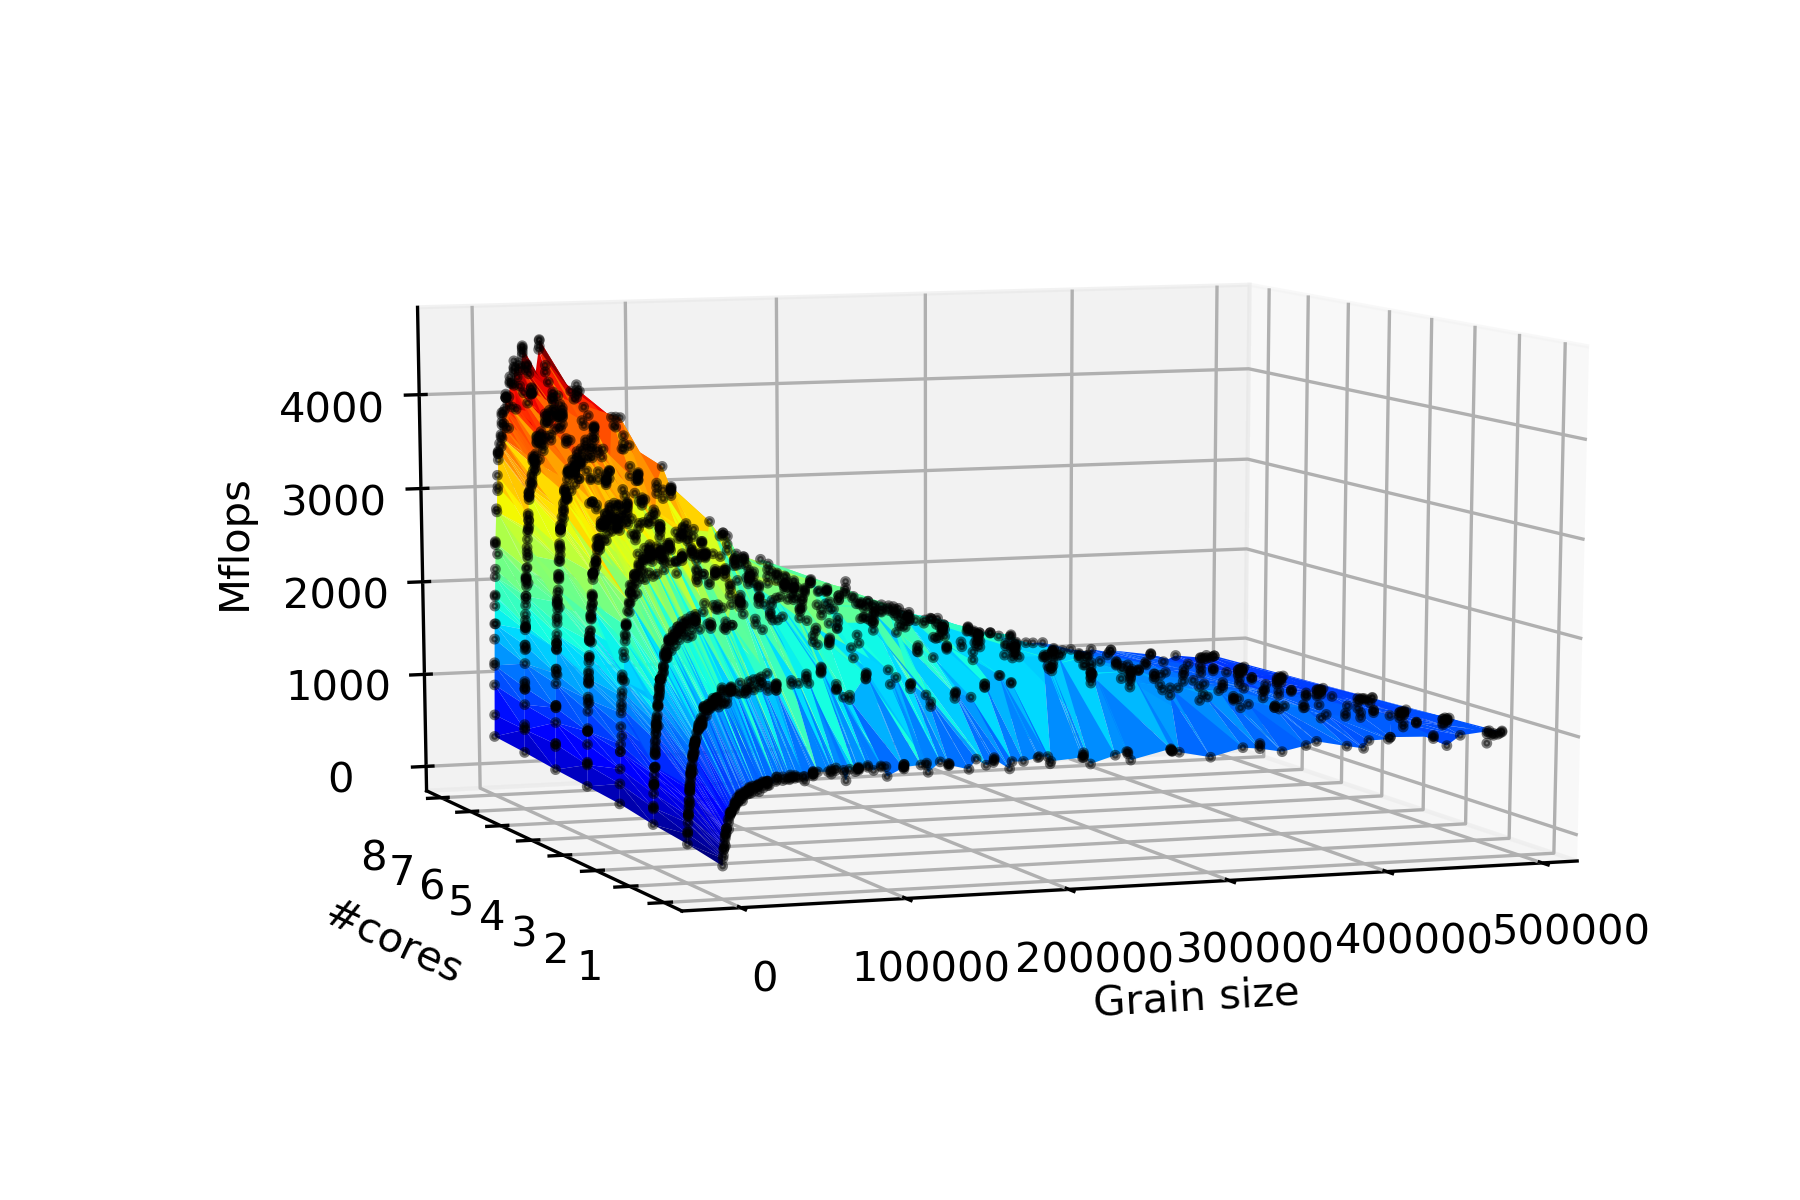
\includegraphics[width=1\linewidth]{images/fig2.png}
	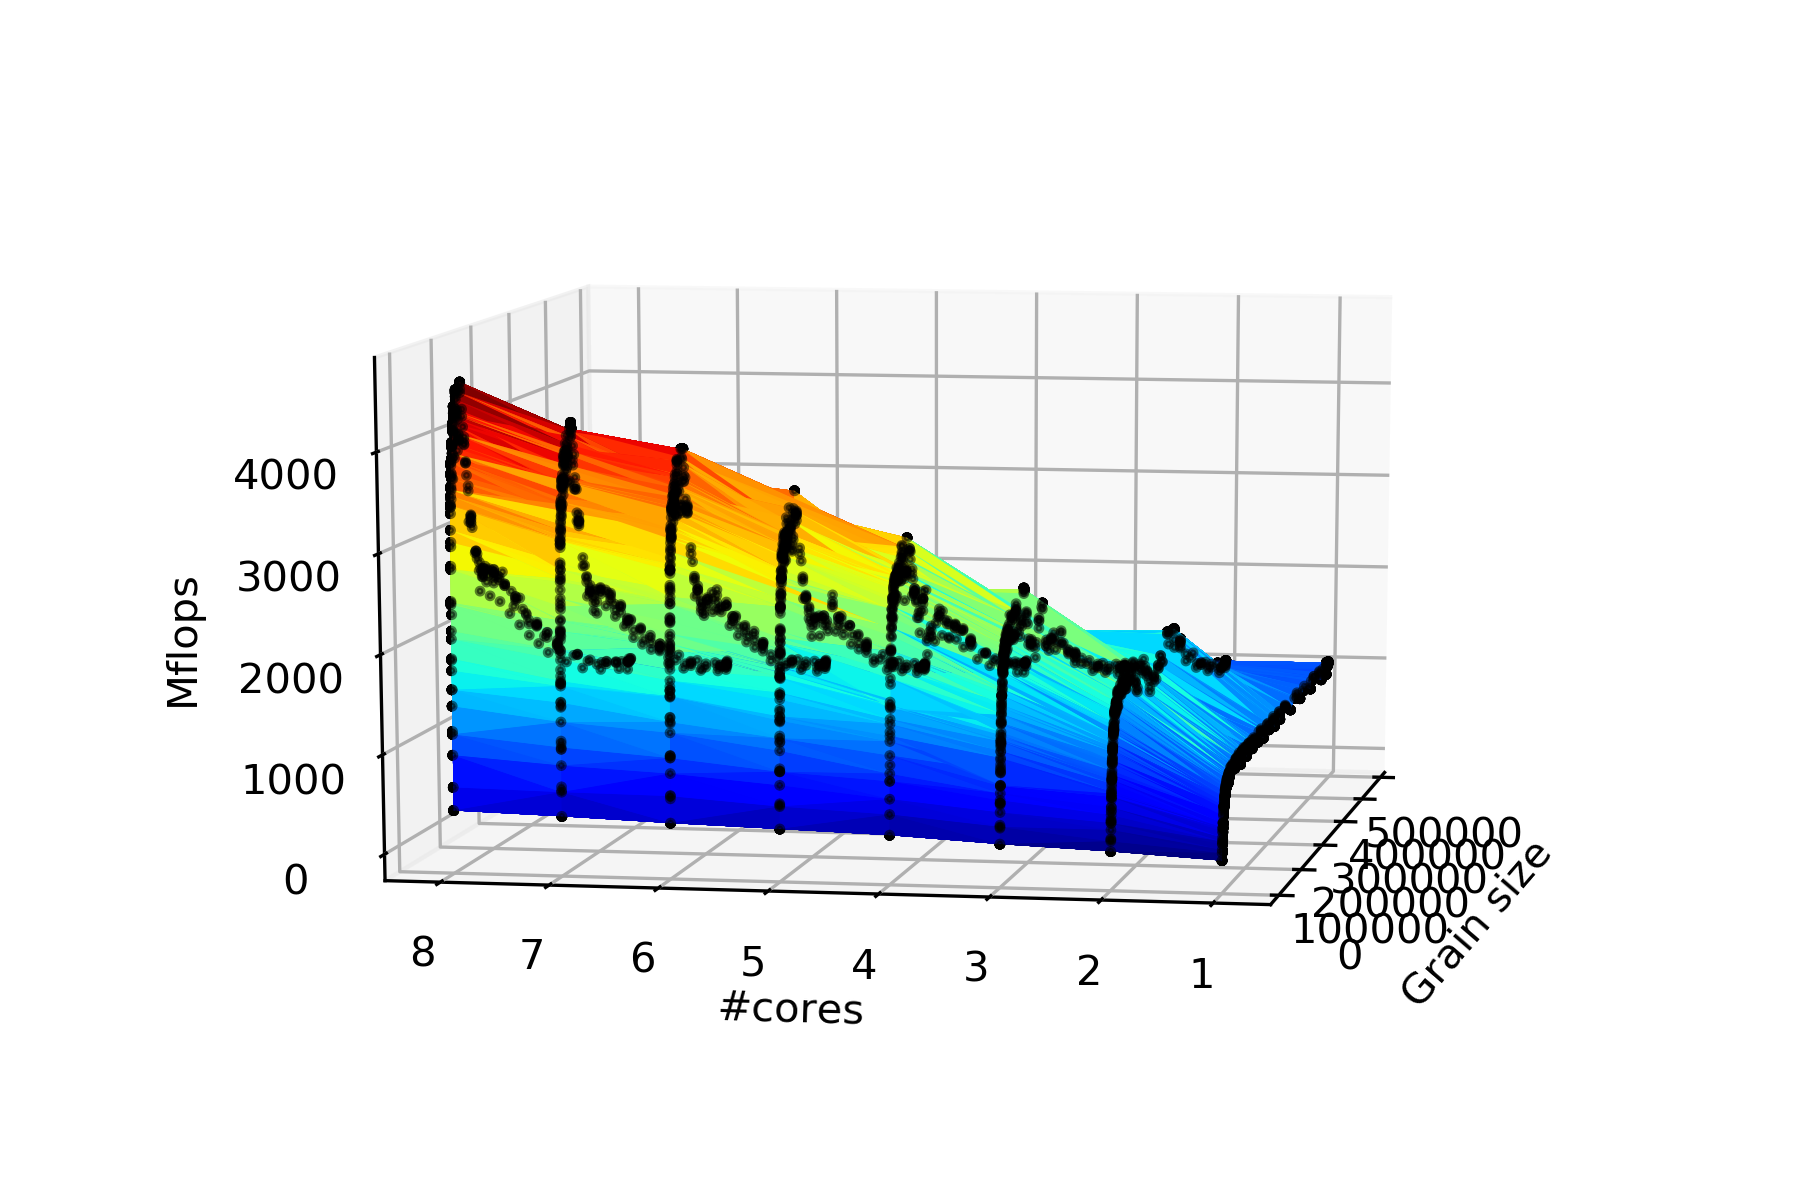
\includegraphics[width=1\linewidth]{images/fig3.png}
	\caption{An example of results obtained from Blazemark running $DMATDMATADD$ benchmark for matrix of size 690$\times$690 from two different angles}	
	\label{fig1}
\end{figure}

\subsection{Observation}

\subsection{L2 cache miss analysis}
In this set of experiments we used the performance counters integrated into HPX to measure the cache miss rate for different grain\textunderscore sizes w

-grain\textunderscore size

\pagebreak

\singlespacing
\chapter{Results}
\doublespacing
\section{Setup}
Marvin:
cache level 1
coherency line size: 64
number of sets: 512
ways of associativity: 8
type: Instruction
size: 32K

cache level 2
coherency line size: 64
number of sets: 512
ways of associativity: 8
type: Unified
size: 256K

cache level 3
coherency line size: 64
number of sets: 512
ways of associativity: 20
type: Unified
size: 20480K


Trillian:
cache level 1
coherency line size: 64
number of sets: 64
ways of associativity: 4
type: Data
size: 16K

cache level 1
coherency line size: 64
number of sets: 512
ways of associativity: 2
type: Instruction
size: 64K

cache level 2
coherency line size: 64
number of sets: 2048
ways of associativity: 16
type: Unified
size: 2048K

cache level 3
coherency line size: 64
number of sets: 2048
ways of associativity: 48
type: Unified
size: 6144K
\pagebreak

\singlespacing
\chapter{Future Plans}
\doublespacing
\input{chapters/06_chapter}
\pagebreak

\singlespacing
\addtocontents{toc}{\vspace{12pt}}
\addcontentsline{toc}{chapter}{\hspace{-1.6em} REFERENCES}
%\begin{thebibliography}{999}
\vspace{0.9em}
\bibliographystyle{unsrt}
\bibliography{bibliography}
%\input{bibliography}
%\end{thebibliography}


\addtocontents{toc}{\vspace{12pt} \hspace{-1.8em} APPENDIX \vspace{-1em}}
\pagebreak

\singlespacing
\appendix
%\chapter{Copyright Information}
%\vspace{0.5em}
%\input{appendixA}
%\pagebreak
%\addtocontents{toc}{\vspace{12pt} \hspace{-1.8em} APPENDIX \vspace{-1em}}
%\appendix
%\chapter{Title of Appendix A}
%\vspace{0.5em}
%\input{appendixA}
%\pagebreak
%\chapter{Title of Appendix B}
%\vspace{0.5em}
%\input{appendixB}
%\pagebreak
%If you need to insert additional appendices, copy the previous four lines, using appendixY as the
%argument of the \input commnd for Appendix Y, for Y=C,D,E,...

%Finally, the vita section is created and included in the Table of Contents.
%\chapter*{Vita}
%\doublespacing
%\setlength{\parindent}{1.75em}
%\vspace{0.2em}
%\addtocontents{toc}{\vspace{12pt}}
%\addcontentsline{toc}{chapter}{\hspace{-1.5em} VITA}
%Insert the text of your vita, which is basically a description of yourself and your academic career.
%\singlespacing
%\chapter*{Vita}
%\doublespacing
%\setlength{\parindent}{1.75em}
%\vspace{0.2em}
%\addtocontents{toc}{\vspace{12pt}}
%\addcontentsline{toc}{chapter}{\hspace{-1.5em} VITA}
%VITA
\end{document}